\chapter{ Констукторский раздел}
\label{cha:design}
    В данном разделе будут рассмотрены схемы алгоритмов, требования к функциональности ПО, и определены способы тестирования.
    
    \section{Требования к функциональности ПО}
        В данной работе требуется обеспечить следующую функциональность.
        \begin{enumerate}
            \item Пользовательский режим:
            \begin{enumerate}
                \item возможность подать на вход массив;
                \item вывод результата корректной сортировки.
            \end{enumerate}
	\item Тестовый режим: 
            \begin{enumerate}
            	\item возможность замера процессорного времени реализации каждой сортировки в худшем, лучшем и произвольном случае;
            \end{enumerate}
        \end{enumerate}
	
	\section{Схемы алгоритмов}
        Ниже будут представлены схемы сортировок: \begin{enumerate}
            \item плавная сортировка (рисунок \ref{schema:SmoothSort_1});
            \item сортировка расчёской (рисунок \ref{schema:CombSort});
            \item сортировка слияением (рисунок \ref{schema:MergeSort}).
        \end{enumerate}
      
       	    \begin{figure}[h!]
       		\centering
       		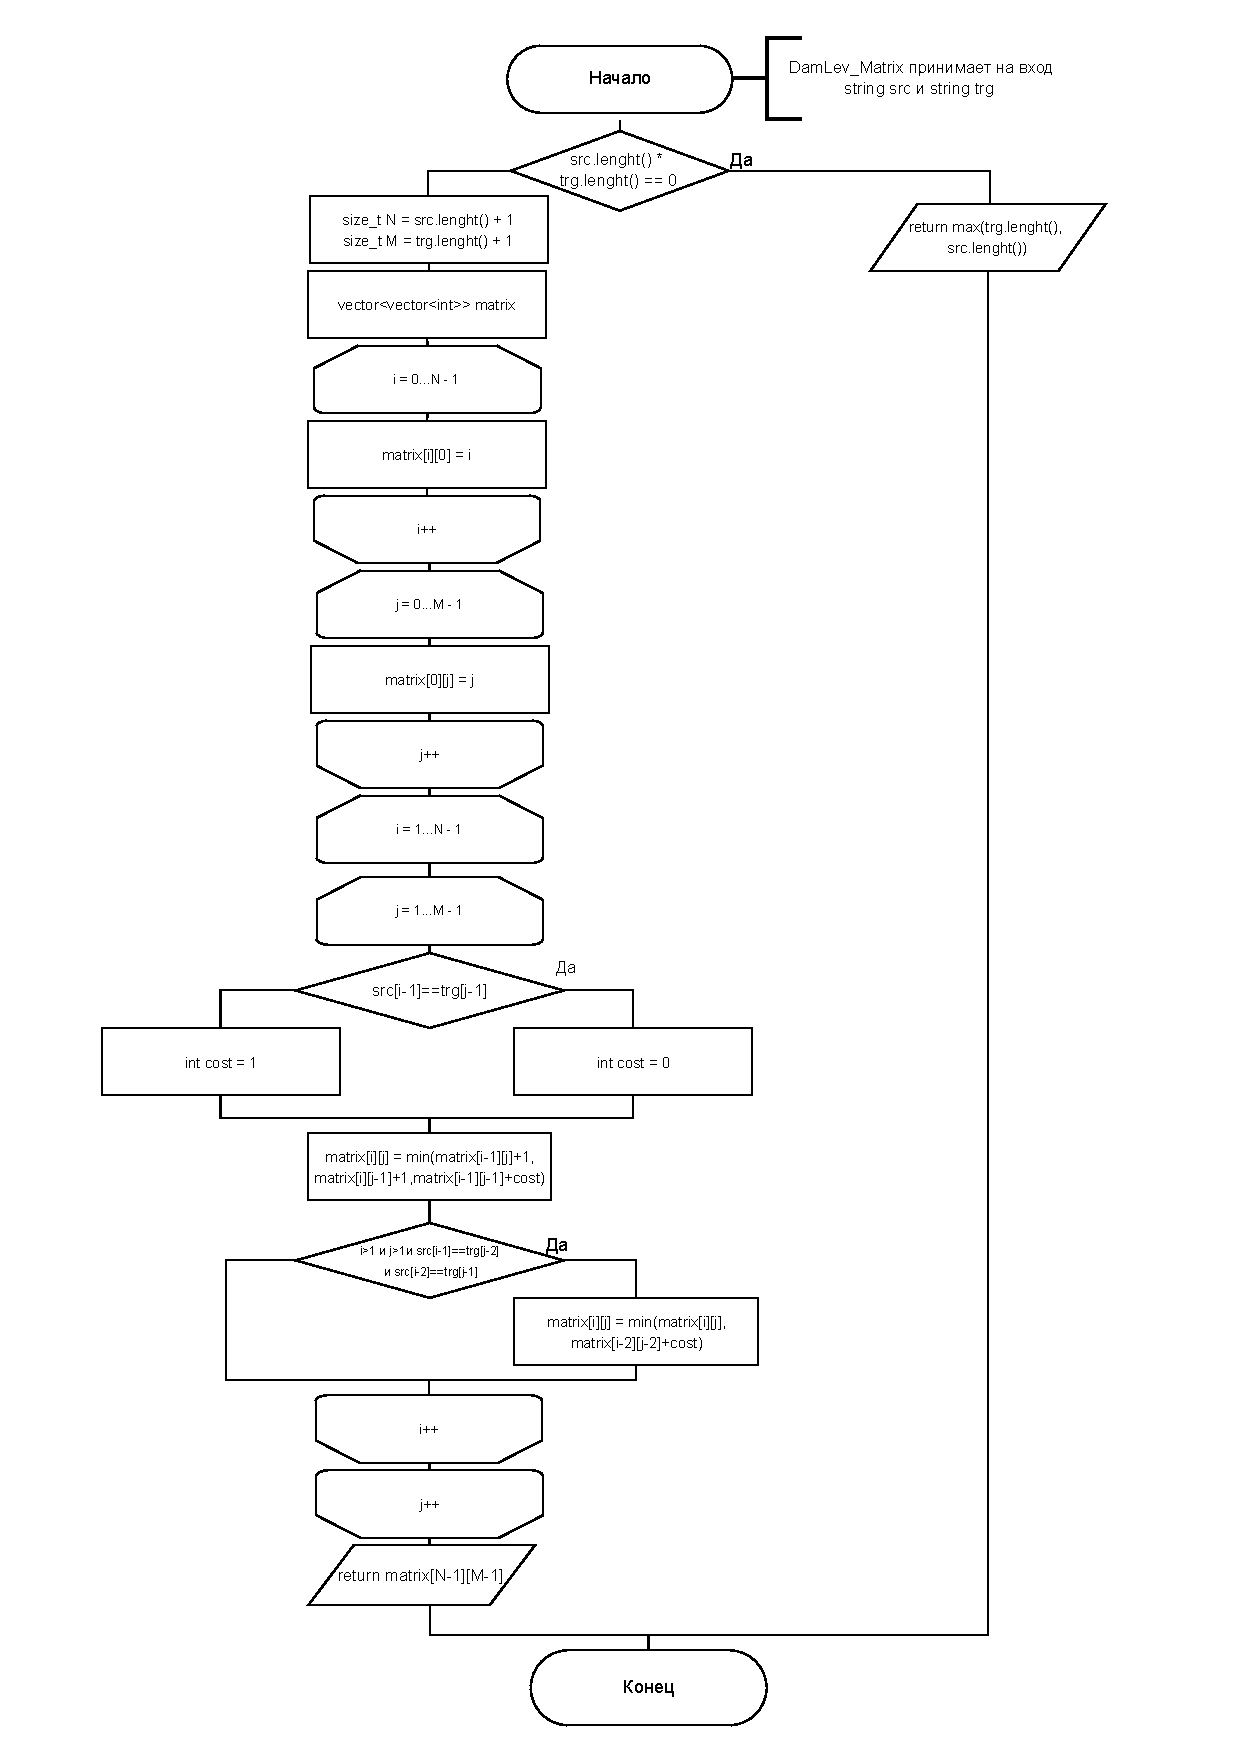
\includegraphics[scale=0.8]{DamLevMatrix.pdf}
       		\caption{Схема нерекурсивного алгоритма нахождения расстояния Дамерау-Левенштейна}
       		\label{schema:matr:DamLevenstein}
       	\end{figure}\clearpage
       	
       	\begin{figure}[h!]
       		\centering
		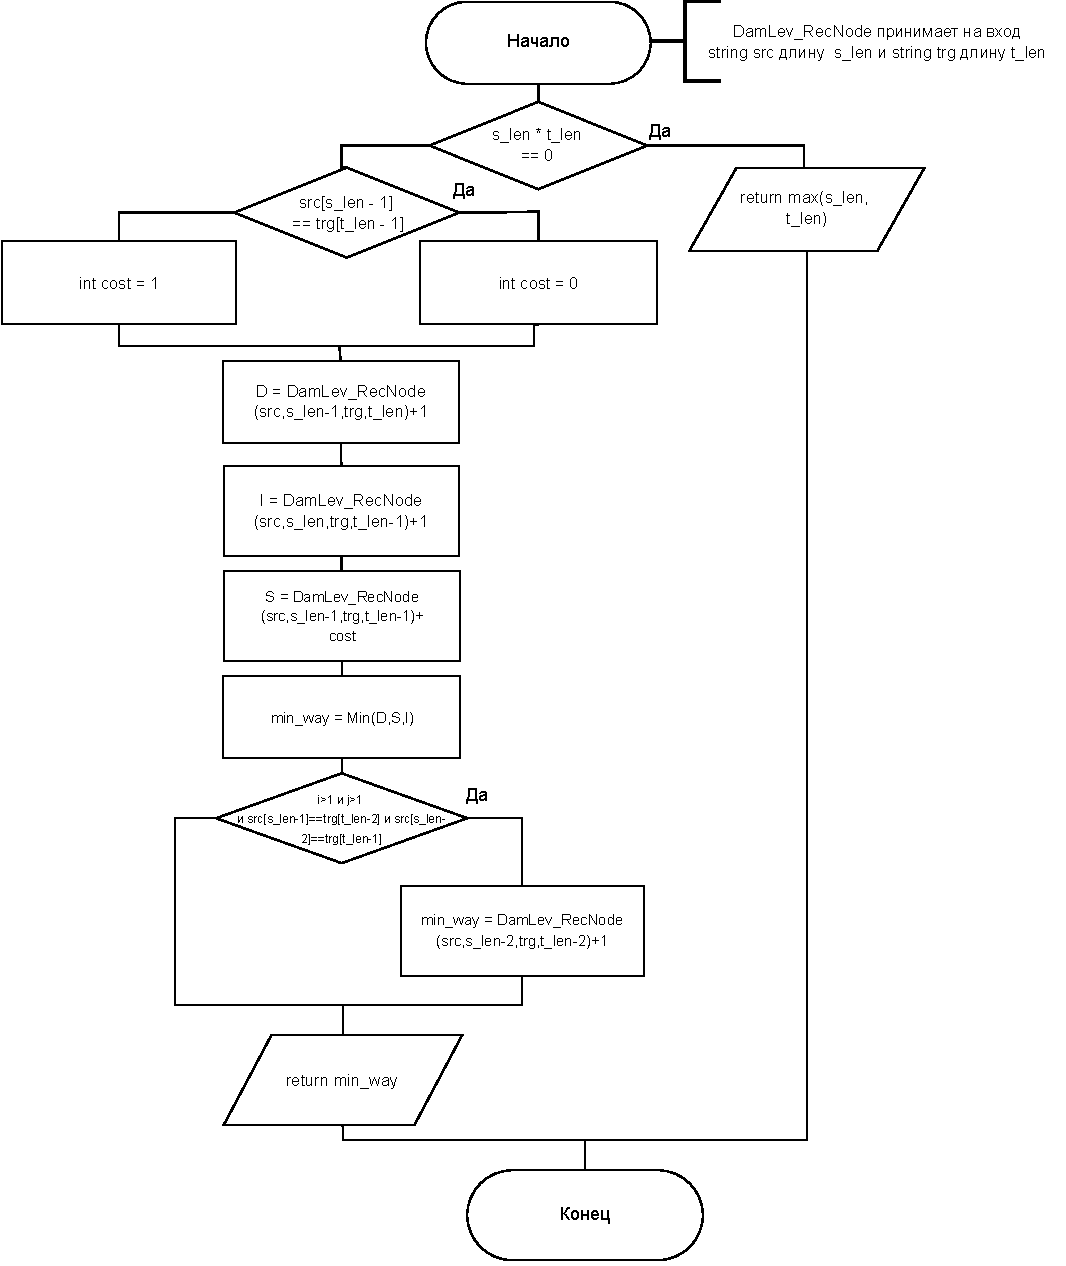
\includegraphics[scale=1]{DamLevRec.pdf}
       		\caption{Схема рекурсивого алгоритма нахождения расстояния Дамерау-Левенштейна}
       		\label{schema:rec:DamLevenstein} 
       	\end{figure}\clearpage
       	
       	\begin{figure}[h!]
       		\centering
		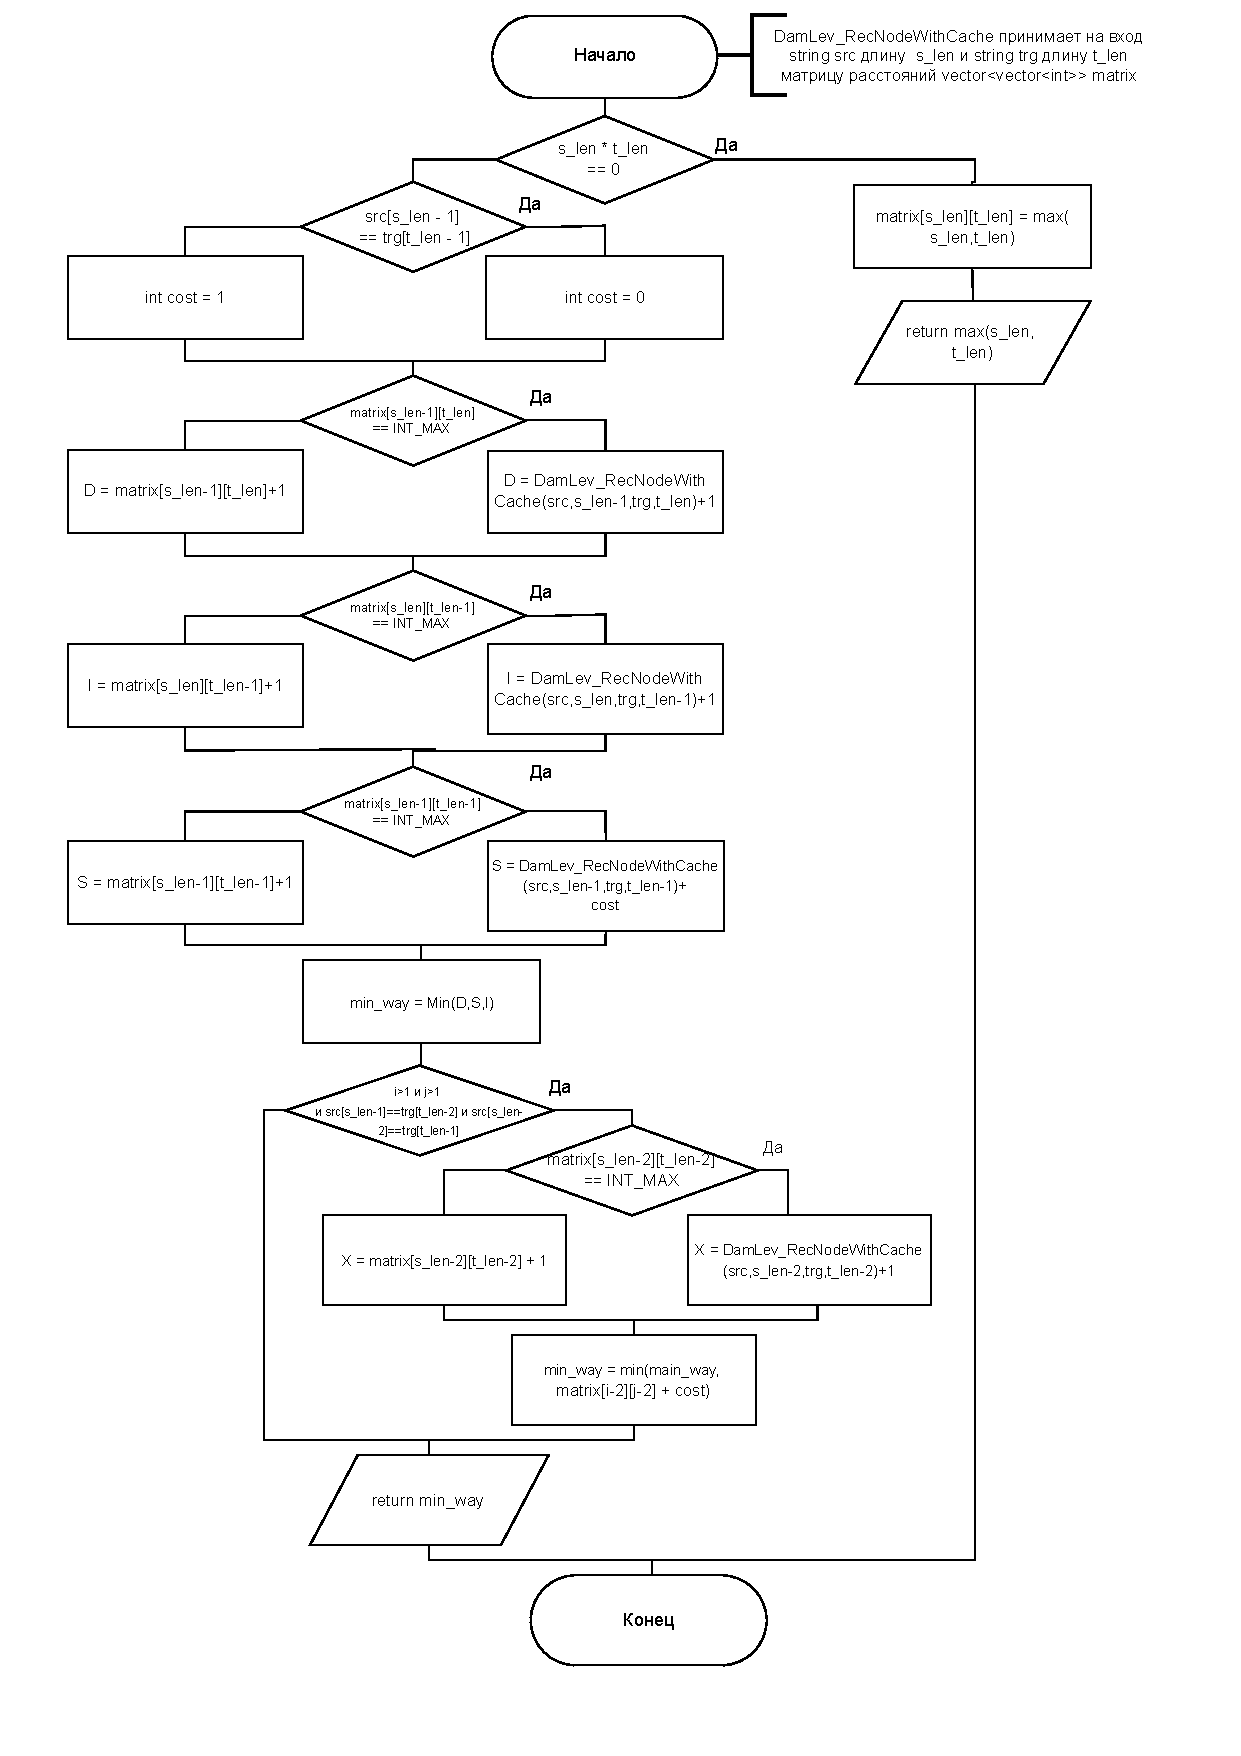
\includegraphics[scale=0.8]{DamLevRecCache.pdf}
       		\caption{Схема рекурсивого алгоритма нахождения расстояния Дамерау-Левенштейна с кэшированием}
       		\label{schema:rec-matr:DamLevenstein}
       	\end{figure}\clearpage
       	
       	\begin{figure}[h!]
       		\centering
		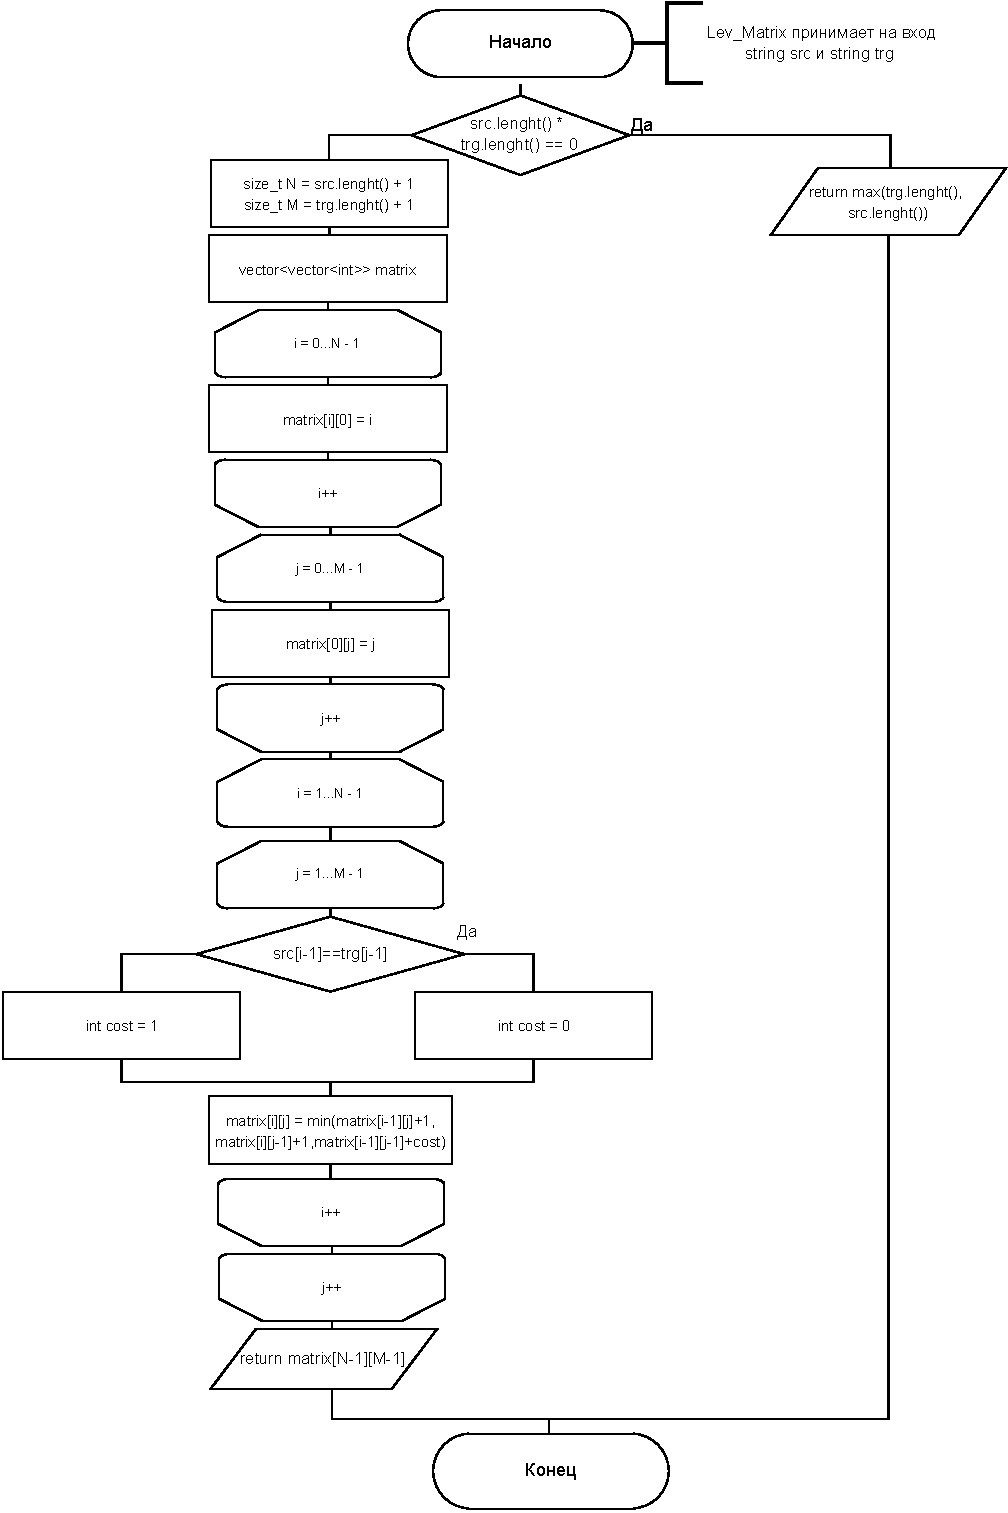
\includegraphics[scale=0.9]{LevMatrix.pdf}
       		\caption{Схема нерекурсивного алгоритма нахождения расстояния Левенштейна}
       		\label{schema:matr:Levenstein}
       	\end{figure}\clearpage

    \section{Требования к функциональности ПО}
        В данной работе требуется обеспечить следующую функциональность.
        \begin{enumerate}
            \item Пользовательский режим:
            \begin{enumerate}
                \item возможность считать две строки;
                \item вывод расстояний Левенштейна и Дамерау-Левенштейна между строками.
            \end{enumerate}
	\item Тестовый режим: 
            \begin{enumerate}
            	\item возможность замера процессорного времени реализации каждого алгоритма для строк, заданнных внутри программы;
            \end{enumerate}
            \item Экспериментальный режим: 
            \begin{enumerate}
                \item вывод графиков с процессорным временем работы алгоритмов для варьирующихся строк.
            \end{enumerate}
        \end{enumerate}
        

    \section{Тесты}
    Тестирование ПО будет проводиться методом чёрного ящика. Необходимо проверить работу системы 
    на тривиальных случаях (одна или обе строки пустые, строки полностью совпадают) 
    и несколько нетривальных случаев.
  	

	\section*{Вывод}


	В данном разделе были разработаны схемы используемых алгоритмов и требования к функциональности программы.
\newpage